\scanpage{23}
\deleted{In the general case (motives not necessarily constant) does knowledge of the operations $\Theta_X$ on the $V_{\mathbb{C}}$ $(V\in\operatorname{Ob}\mathcal{M})$ imply that of the elements of the structures $1^{\mathrm o}$ and $2^{\mathrm o}$, \deleted{or at least to what extent?}}
\margin{\deleted{\uuline{yes}} ??}

\margin{\begin{tikzpicture}
\node[inner sep=1pt,align=left,text width=.93\marginparwidth] (rubrique) {Abstract situation of the datum of an integrable connection a fibre functor.};
\draw (rubrique.north west) -- (rubrique.south west) -- (rubrique.south east);
\end{tikzpicture}}

\begin{center}\rule[.2ex]{2cm}{.4pt}\end{center}

Consider a $\otimes$-category $\mathcal{M}$ over a field $k_0$, let $K$ be an extension of $k_0$. We suppose given a fiber functor with values in $k_0$, \unsure{thus|in} $\mathcal{M}$. with this fiber functor is given by $G$ over $k_0$, $\mathcal{M}$ identifies with \unsure{``$G$-$k_0$-modules\ldots|$G$-$k_0$-modules\ldots} We want to determine the ways of putting, on each $V\otimes_{k_0}K$ an integrable connection \inserted{relative to : $K/k_0$}, \uline{functorial} in $V$, \inserted{and ``compatible with $\otimes$''.}

Now there is already one $\unsure{\Theta_0|\text{\textcircled{H}}_0}$, derived from the $k$-structures which we \deleted{\unsure{suppose}} already have on each $V\otimes_{k_0}K$. Another connection \deleted{\unsure{integrable}} \inserted{on $V$} will therefore be of the form
\[
 \Theta_X^V={\Theta_0}_X^V+\omega^V(X)^{\deleted{\unsure{V|x}}}
\]
\unsure{where|or}
\[
 \omega^V\deleted{\unsure{(X)|\in}}:\operatorname{Dér}_{k_0}(K/k_0)\longrightarrow
 \operatorname{End}_K(V_K\unsure{)}\,\text{is \uline{$K$-linear}}
\]
\[
 \Theta_X^V(\varphi)={\Theta_0}_X^V(\varphi)+\omega^V(X)(\varphi)
\]
If we want to choose the $\Theta_X^V$ for every $V$, in a way compatible with multiplication, we find that \deleted{$\unsure{\omega^V|\omega}\unsure{\Theta_X|(X)}$} $\omega^V(X)$, for variable $V$, is a ``derivation'' of the fiber functor \deleted{\unsure{given}}\inserted{$F_K$}, thus defined by an element of \deleted{Lie} $\mathfrak{g}_K$, where $\mathfrak{g}=\operatorname{Lie}G$. Let $\omega(X)\in\mathfrak{g}_K$ be this element.
% archive sheet number: 22
